\chapter{The second chapter}\label{chap2}
{
\hypersetup{linkcolor=\linkColor}
\minitoc
}
\newpage

% Uncomment the line below if you do not want to print headers in the first
% chapter page
% \thispagestyle{plain}

\begin{refsegment}

\section{First section of chapter 2}\label{sec:chap2.sec1}

Here I am going to insert a picture of my cat.

\begin{figure}[H]
    \centering
    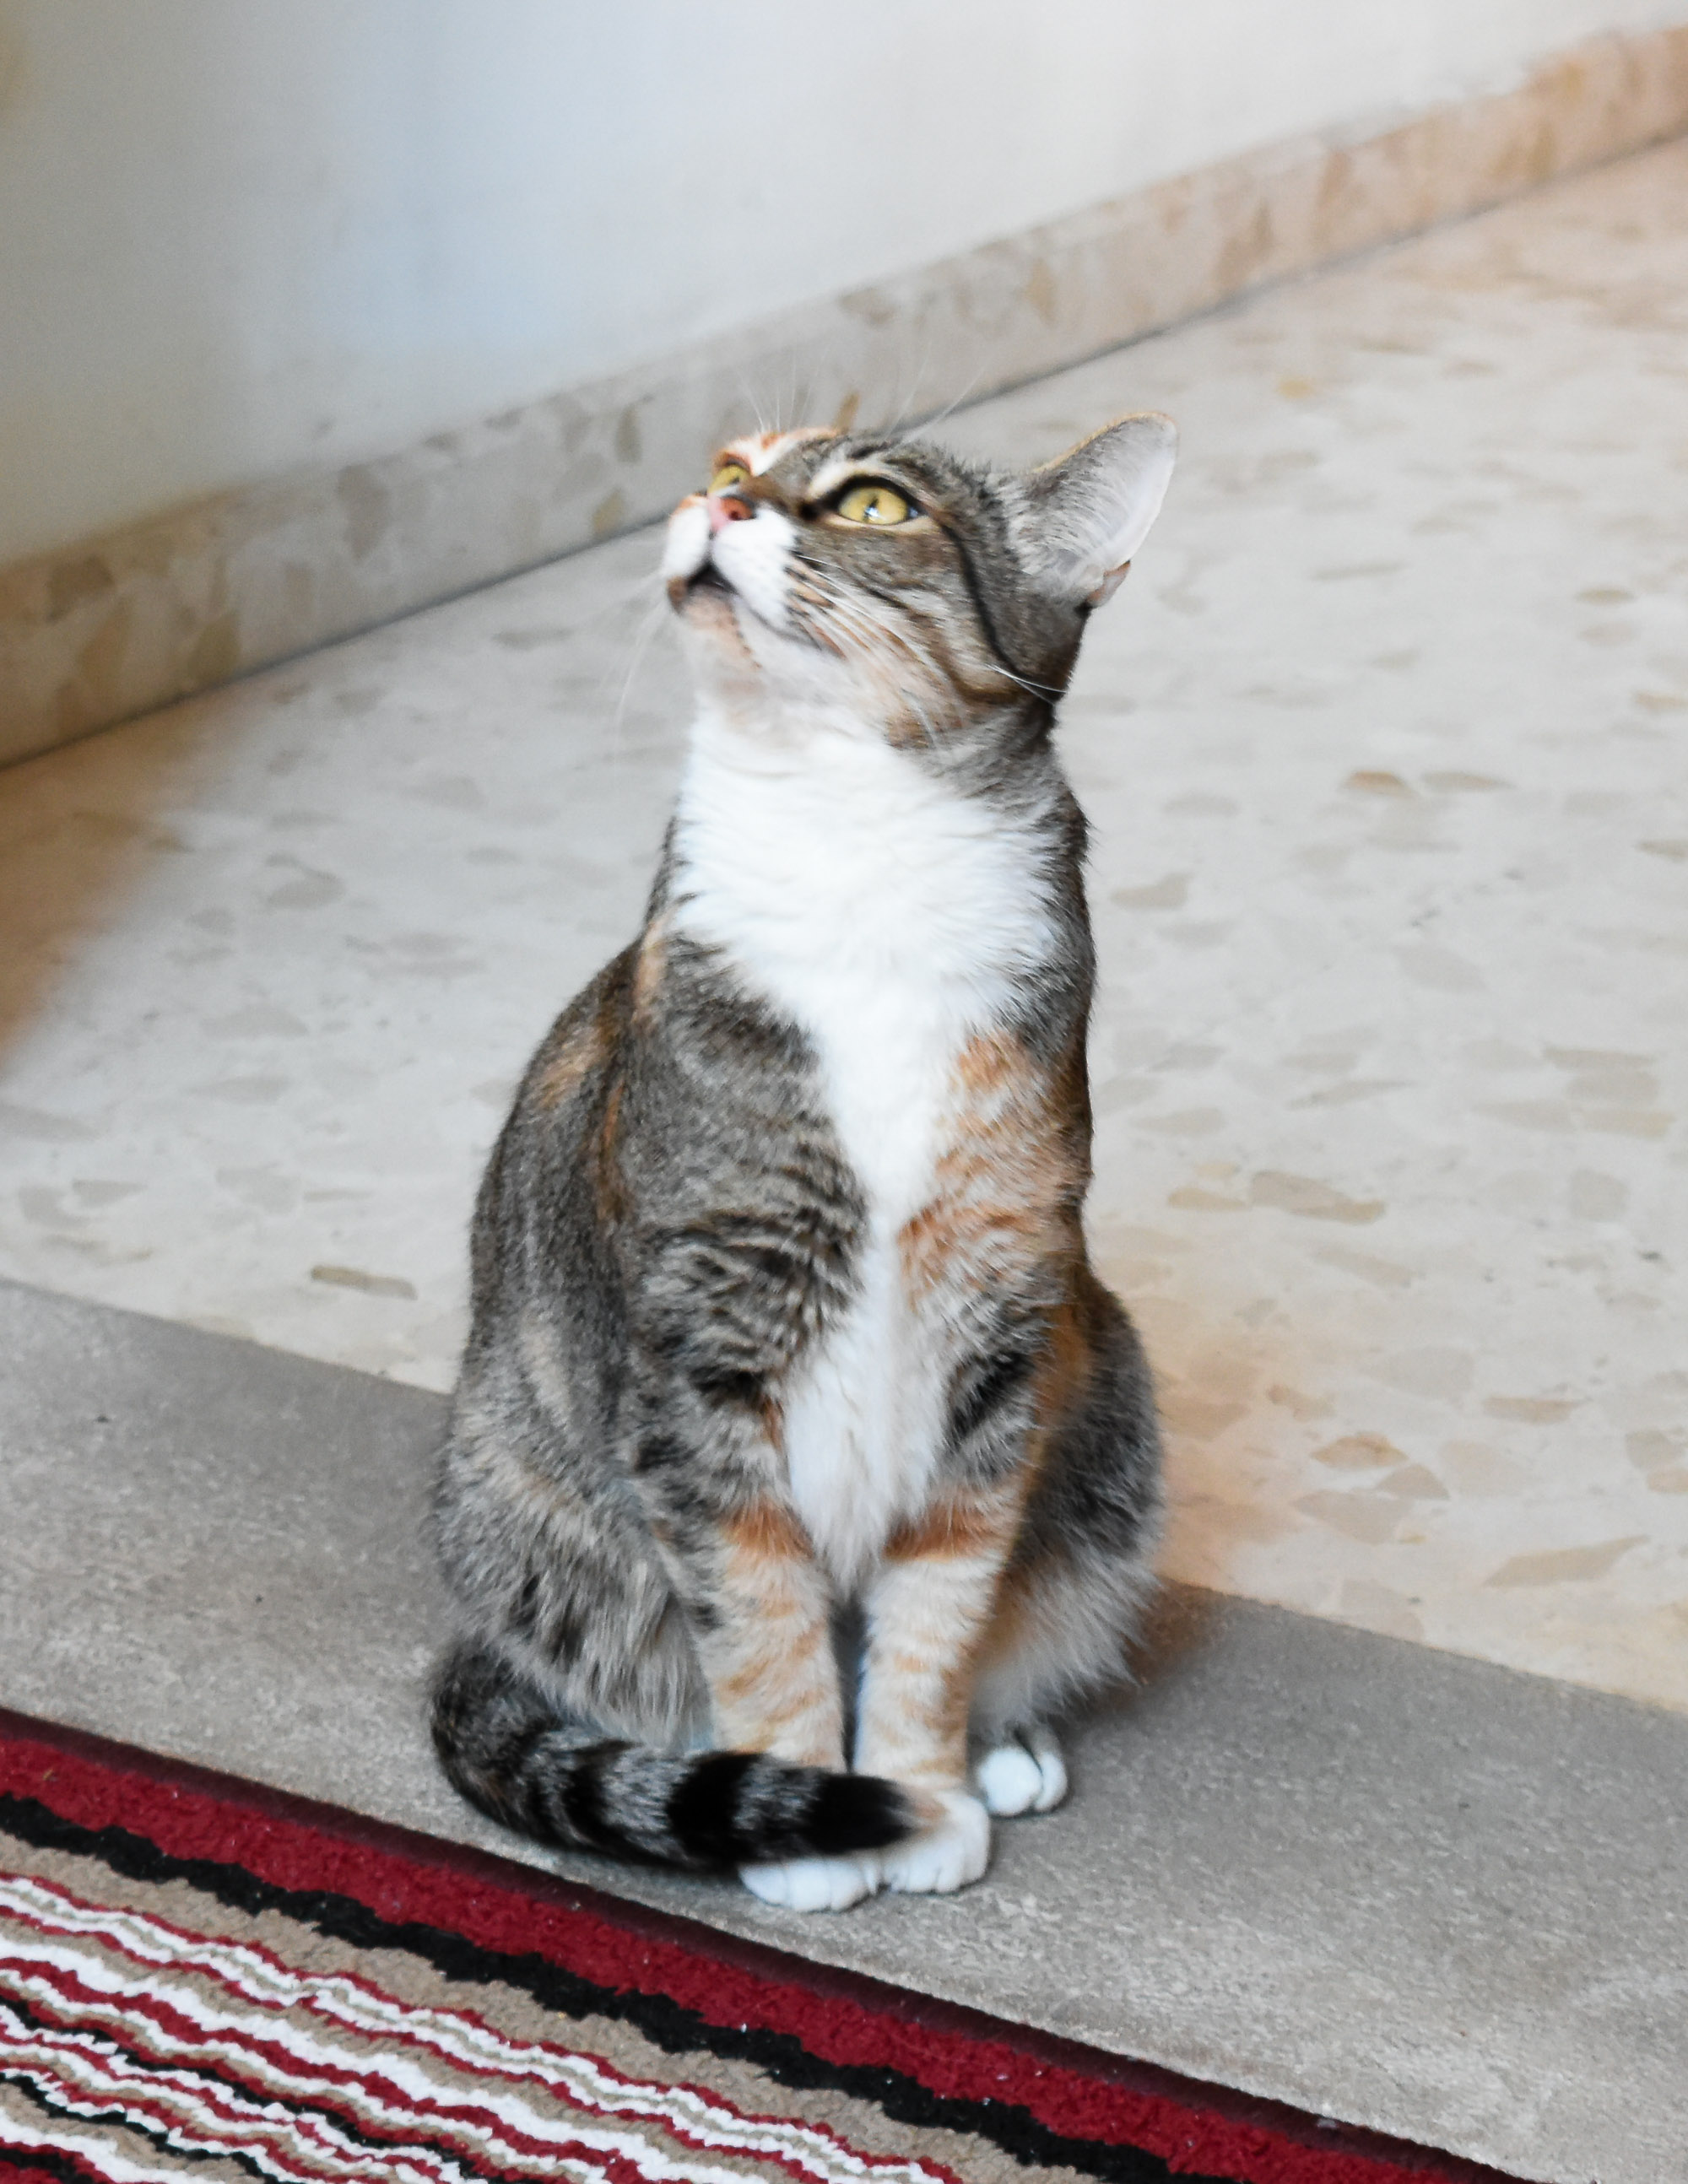
\includegraphics[width=0.9\textwidth]{./chapter_2/figures/Greta.jpg}
    \caption{She is Greta.}
    \label{fig:Greta}
\end{figure}

Some maths!

\blindmathtrue
\blindmathpaper
\blindmathfalse

\section{Second section of chapter 2}\label{sec:chap2.sec2}

Another citation \cite{dummyArticle}

\noindent And a table, using my font for displaying numbers. 

\begin{center}
    \begin{table}[h!]
        \begin{longtable}{lll}
            \textit{Letter} & \textit{Type} & \textit{Value}\\
            A & vowel & \numbersfont{23} \\
            D & consonant & \numbersfont{35} \\
            F & consonant & \numbersfont{66} \\
            J & consonant & \numbersfont{41} \\
            O & vowel & \numbersfont{20} \\
            \caption{A table using two fonts.}
        \end{longtable}
    \end{table}
\end{center}

\newpage

% Load custom header for references section
%*****************************************************************************%
%******************* HEADER & FOOTER - BIBLIOGRAPHY PAGE *********************%
%*****************************************************************************%

\pagestyle{fancy}
\fancyhf{} % removes current header and footer

%********************************** HEADER ***********************************%

% Undo chapter and section automatic uppercase
\renewcommand{\chaptermark}[1]{ \markboth{#1}{}}
\renewcommand{\sectionmark}[1]{ \markright{#1}{}}

% Section name on right side in odd pages
\fancyhead[RO]{\slshape{\textcolor{\accentColor}{\textbf{\Large{\thesection}}%
}\, \textup{|} \, \mdseries \sectionfont References}}
% Chapter name on left side in even pages
\fancyhead[LE]{\slshape{\textcolor{\accentColor}{\textbf{\chaptername\:\Large%
{\thechapter}}} \, \textup{|}  \, \mdseries \sectionfont\leftmark}}

% Information:
% - \thepage     -> number of the current page
% - \leftmark    -> current chapter name printed like "CHAPTER 3. THIS IS THE
%                   CHAPTER TITLE"
% - \rightmark   -> current section name printed like "1.6. THIS IS THE SECTION
%                   TITLE"
% - \chaptername -> the name chapter in the current language. If this is
%                   English, it will display "Chapter"
% - \thechapter  -> current chapter number
% - \thesection  -> current section number 

\renewcommand{\headrulewidth}{0cm} % Removes division line in the header

%********************************** FOOTER ***********************************%

% Page number on right side in odd pages
\fancyfoot[RO]{\slshape{\sectionfont Page} \textcolor{\accentColor}{\bfseries%
\Large\thepage}}
% Page number on left side in even pages
\fancyfoot[LE]{\slshape{\sectionfont Page} \textcolor{\accentColor}{\bfseries%
\Large\thepage}}

\printbibliography[segment=1,heading=subbibliography]
% Attach this references section to the chapter mini-TOC
\addcontentsline{toc}{section}{Chapter 2 References}

% Do not forget to close the refsegment
\end{refsegment}
